\documentclass[a4]{jgaa-art}

\usepackage{graphicx}
\usepackage{amsmath}
\usepackage{amssymb}
\usepackage[toc,page]{appendix}
\usepackage{caption}
\usepackage{subcaption}
\usepackage{algorithm}
\usepackage[noend]{algpseudocode}
\usepackage{hhline}
\usepackage{array}
\newcolumntype{C}[1]{>{\centering\let\newline\\\arraybackslash\hspace{0pt}}m{#1}}

\newenvironment{definition}[1][Definition]{\begin{trivlist}
\item[\hskip \labelsep {\bfseries #1}]}{\end{trivlist}}

\makeatletter
\def\BState{\State\hskip-\ALG@thistlm}
\makeatother

\algnewcommand{\LineComment}[1]{\State \(\triangleright\) #1}

\title{Enhancing PQ-tree Planarity Algorithms for non-adjacent $s$ and $t$ }

\author{Shoichiro Yamanishi}

\date{\today}

\begin{document}

\maketitle

\begin{abstract}
The PQ-tree based planarity testing algorithm presented
by Booth and Lueker in \cite{BL76} requires an st-ordering where $\{s,t\}$ must exist.
We propose an enhancement to the algorithm that permits st-ordering of any vertex pair.
The enhancement is made by introducing a type of circular consecutiveness of pertinent 
leaves denoted by  {\it complementarily partial},
 where the pertinent leaves can be consecutively arranged only at both ends of the frontier with 
one or more non-pertinent leaves in between. 
The implementation is enhanced with 4 additional templates P7, P8, Q4, and Q5.
The correctness of the new algorithm is given following the proof in
 \cite{EVEN79} and \cite{LEC67} 
on the equivalence of PQ-tree and its new reduction operations to the corresponding bush form.
The complexity of the new algorithm stays $O(|N|)$.
\end{abstract}

\section{Introduction}\label{se:intro}

%Context
%Purpose
%Summary
%Forecast

PQ-tree data structure and the reduction algorithm were first proposed by Booth and Lueker \cite{BL76} 
in 1976.
PQ-tree is a rooted ordered tree with three node types: L-node represents a leaf with no children, P-node 
permits any permutation of its children, Q-node has an ordering on its children but it can be reversed.
PQ-tree is used to represent a set of permissible permutations of elements in $S$, and the reduction
operation tries to find a consecutive arrangement of subset $U$ of $S$.
It has many applications including the planarity testing of an undirected biconnected graph $G(V,E)$.
Booth and Lueker proposed a planarity testing algorithm in their original paper \cite{BL76}.
It has $O(|N|)$ time complexity, and it depends on a particular ordering on graph vertices called st-ordering,
where the two terminal nodes $s$ and $t$ must be adjacent as in $\{s,t\}$.
An st-ordering can be found in $O(|N|)$ time with an algorithm such as \cite{TARJAN86}, assuming $|E| \le 3|V| - 6$ .

The algorithm falls in a category called vertex addition.
Each graph vertex $v$ is processed in an iteration according to the st-ordering.
Conceptually each graph vertex is added to the bush form \cite{LEC67},\cite{EVEN79}, and the PQ-tree
evolves reflecting the state of the bush form.
Each iteration of the algorithm transforms the PQ-tree for $v$
 and its incident edges.
In the beginning of an iteration, the tree leaves that correspond to the incoming graph edges incident to $v$,
or {\it pertinent leaves}, are gathered consecutively in the tree by transforming the tree 
in a series of template applications.
The minimum connected subtree for all the pertinent leaves, or {\it pertinent tree}, is removed from the tree, 
and then new leaves that corresponds to the outgoing graph edges incident to $v$ are added to the tree node 
that was the pertinent tree root.
The st-ordering ensures there is at least one incoming graph edge and one out going graph edge at 
each iteration except for the first and the last. 
At the first iteration the leaves for the outgoing graph edges of the first graph vertex in the st-ordering
are attached to the initial P-node, and the PQ-tree evolves form there over the iterations.
At an iteration, if the pertinent leaves can not be arranged consecutively, the algorithm aborts and declares it
non-planar.
At the second to last iteration, if all the pertinent leaves are consecutively arranged, the graph is declared planar.

The PQ-tree itself is an elegant data structure to represent a set of permissible permutations of elements, 
but its reduction algorithm involves 10 rather cumbersome tree transformation operations called templates, though
each of them is straightforward and intuitive to understand.
Since the original algorithm was published, many graph planarity-related algorithms have been proposed,
 but some of them were later proven to have some issues in them \cite{OZAWA81} \cite{JTS89} \cite{KANT92}.
For example, J\"unger, Leipert, and Mutzel \cite{JUNGER97} discuss the pitfalls and difficulties of using 
PQ-trees for maximal planarization graphs.
It seems to take a very careful attention when we apply PQ-tree to graph planarity algorithms despite its apparent 
straight-forwardness and intuitiveness.

Another data structure called PC-tree was proposed by Shih and Hsu \cite{HSU99}.
It is a rootless tree to express permissible 'circular' permutations. 
Hsu \cite{HSU99} proposes a planarity test algorithm using PC-tree with iterative vertex
 addition along a DFS exploration of graph vertices.
Hsu \cite{HSU01} compares PQ-tree and PC-tree in terms of planarity testing. 
Hsu\cite{HSU01} mentions testing 'circular ones' property with PC-tree and 
'consecutive ones' property with PQ-tree.

In this paper, we will expand the PQ-tree planarity algorithm for any (not necessarily adjacent) $s$,$t$ pair.
A non-adjacent st-ordering will introduce a new type of consecutiveness through the course of the algorithm on the PQ-tree.
It is a type of 'circular' permutation.
We define the type of circular permutations that the original algorithm can not handle 
 as {\it complementarily partial}. 
We show the insufficiency of the set of the original templates in Booth and Lueker \cite{BL76} with a specific example, and propose 4 
new templates to handle complementarily partial nodes.
Then we prove the correctness of the new algorithm following  Lempel, Even, and Cederbaum \cite{LEC67} and Even \cite{EVEN79} in equivalence to the corresponding bush form. 
We show the time complexity stays $O(|N|)$. 
We then discuss some implementation details.
The algorithm mainly consists of two parts called BUBBLE() and REDUCE() in \cite{BL76}.
We show that no change is required for BUBBLE(), but the 4 new templates have to be added to REDUCE().

PQ-tree and its reduction technique are also used for some planarization algorithms such as
\cite{OZAWA81}, \cite{JTS89}, and \cite{KANT92}.
In those algorithms, the costs are calculated per tree node, 
and some tree leaves that have associated graph edges are removed based on the costs to maintain planarity.
The costs are basically the number of descendant tree leaves that would have to be removed to 
make the tree node of certain pertinent and non-pertinent type.
We briefly propose an improvement on the cost values.
Without the improvement, some graph edges can be removed unnecessarily as a consequence of lack of handling the {\it complementarily partial} nodes defined below.


\section{Circular Consecutiveness}\label{se:insuff}

The insufficiency of the existing algorithm is best shown by a real example.
Please see figure~\ref{fig:pq_tree_01} and~\ref{fig:bush_form_01}.
They are taken from a snapshot of the original algorithm for the graph and the st-numbering shown in Appendix A.
Figure~\ref{fig:pq_tree_01} is the PQ-tree at the 23rd iteration after 
BUBBLE(), and figure~\ref{fig:bush_form_01} is the corresponding bush form.
In this iteration the graph vertex $2$ is to be added.
The pertinent leaves that correspond to $\{8,2\}$,$\{3,2\}$, and $\{7,2\}$
 are about to be consecutively arranged in REDUCE().
Those edges can be consecutively arranged in a circular manner.
However, the reduction fails at Q-node $Q4$ as none of the templates Q1,Q2, 
or Q3 can handle this arrangement.
In $Q4$, the pertinent leaves can only be arranged consecutively
 at both ends with one or more non-pertinent leaves in between.

As shown above, the original algorithm is not capable of handling this type 
of arrangements of the pertinent leaves with pertinent leaves at both ends.
This is a result of using a rooted tree structure to handle circular 
consecutiveness around the outer face of the corresponding bush form. 
Once a Q-node has formed in the PQ-tree, at a later iteration 
if there is a pertinent node of complementarily partial, 
there will be no way to arrange the pertinent nodes consecutively using the 
original set of templates, 
even if the corresponding bush form permits circular consecutiveness.


\begin{figure}[!htb]
  \centering
  \begin{minipage}[b]{0.64\textwidth}
    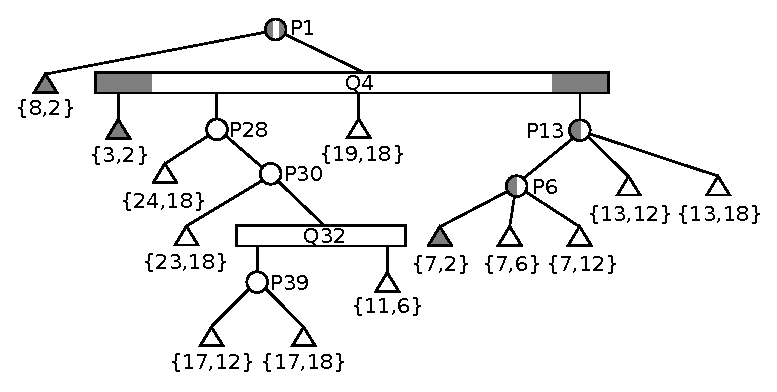
\includegraphics[width=\textwidth]{pq_tree_sample_01}
    \caption{PQ-tree}
    \label{fig:pq_tree_01}
  \end{minipage}
  \hfill
  \begin{minipage}[b]{0.35\textwidth}
    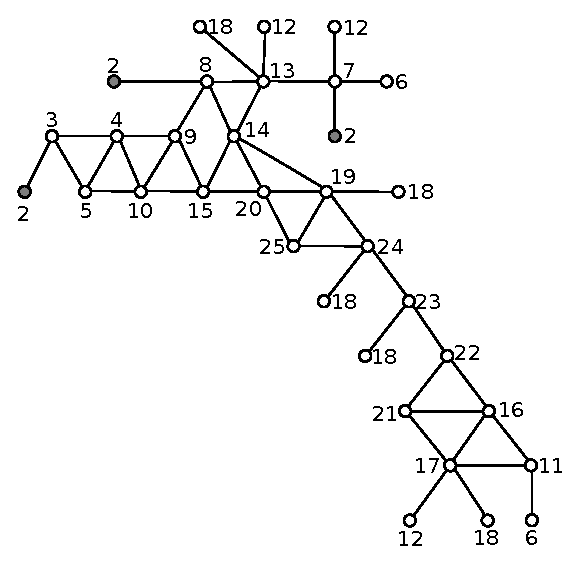
\includegraphics[width=\textwidth]{bush_form_01}
    \caption{Bush form}
    \label{fig:bush_form_01}
  \end{minipage}
\end{figure}


\section{Enhancement with New Templates}\label{se:correction}
In the previous section we showed a type of node arrangement in PQ-tree that
the original algorithm can not handle.
In this section we first formulate this condition by defining a new
pertinent node type {\it complementarily partial}, and then
introduce 4 new templates.
Then we discuss other changes required in BUBBLE() and REDUCE().

\begin{definition}
A \emph{P-node} is \emph{complementarily partial}, if either of the following
holds:
\begin{enumerate}
\item \label{item:P2}It is not a pertinent root, and it satisfies the
condition for template $P6$ on the arrangement of child nodes,
i.e., if there are exactly two singly partial children. (Figure \ref{fig:pq_tree_02})
\item \label{item:P1}There is exactly one complementarily partial child, and all the
 children are full. (Figure \ref{fig:pq_tree_03})
\end{enumerate}
\end{definition}

\begin{definition}
A \emph{Q-node} is \emph{complementarily partial}, if either of the following
holds:
\begin{enumerate}
\item \label{item:Q2}The children are arranged as the complement of permissible arrangement
   for template $Q3$, i.e., if the descendant pertinent leaves can be arranged 
   consecutively at both ends with one or more non-pertinent leaves in between.
 (Figure \ref{fig:pq_tree_04})
\item \label{item:Q1}There is exactly one complementarily partial child, and all the children
   are full
 (Figure \ref{fig:pq_tree_05})
\end{enumerate}
\end{definition}

\begin{figure}[!htb]
  \centering
  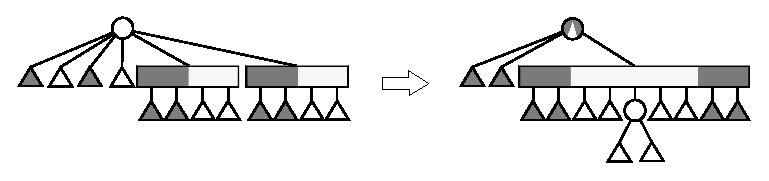
\includegraphics[width=0.9\textwidth]{pq_tree_sample_02}
  \caption{P-node Condition 1, Template P7}
  \label{fig:pq_tree_02}
\end{figure}

\begin{figure}[!htb]
  \centering
  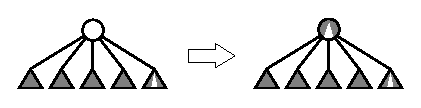
\includegraphics[width=0.5\textwidth]{pq_tree_sample_03}
  \caption{P-node Condition 2, Template P8}
  \label{fig:pq_tree_03}
\end{figure}

\begin{figure}[!htb]
  \centering
  \includegraphics[width=\textwidth]{pq_tree_sample_04}
  \caption{Q-node Condition 1, Template Q4}
  \label{fig:pq_tree_04}
\end{figure}

\begin{figure}[!htb]
  \centering
  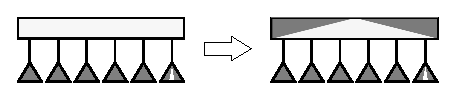
\includegraphics[width=0.55\textwidth]{pq_tree_sample_05}
  \caption{Q-node Condition 2, Template Q5}
  \label{fig:pq_tree_05}
\end{figure}


The first condition for Q-node is formerly defined using a regular expression 
for the children as:
\[F+((S(D?|E+D))|(E+D))|SE*D\]

where $F$ denotes a full child, $S$ a singly partial child, $E$ a 
 non-pertinent child, and $D:=((F|S)F*)$ for notational convenience.

First we show there is no need to change BUBBLE() to handle the complementarily
 consecutive cases.
If the PQ-tree permits complementarily partial arrangement, then the tree
node will be the pertinent tree node. During BUBBLE(), the parent of
all the pertinent nodes will be eventually found, and there will be no need
for a surrogate parent, or {\it pseudo node} in \cite{BL76}.

Next, we introduce 4 new templates for each of 4 conditions shown in the
 definitions above. Basically Template P7 is a complement version of Template P6,
and Template Q4 is a complementary version of Q3. Template P8 and Q5 are
for trivial recursive cases.

Finally we show the updated REDUCE().


\begin{algorithm}
\caption{Template P7}\label{template_P7}
\begin{algorithmic}[1]
\Procedure{TemplateP7}{X: reference to a node object}
\If {$X.type \ne P$} \Return false
\EndIf
\If {Number of singly partial children $\ne 2$} \Return false
\EndIf
\State $newX \gets \text{CreateNewPNode()}$
\State Move all the full children of $X$ to $newX$
\State $C_1 \gets \text{Singly partial child}_1$
\State $C_2 \gets \text{Singly partial child}_2$
\State Remove links of $C_1$ and $C_2$ from $X$
\LineComment At this point $X$ contains zero or more empty children only.
\State Save the location of $X$ in the PQ-tree to $L_X$
\State Unlink $X$ from the PQ-tree
\If {Number of empty children of $X > 1$}
\State Put $X$ to the empty side of sibling list of $C_1$
\ElsIf {Number of empty children of $X = 1$}
\State Put the empty child to the empty side of sibling list of $C_1$
\State Discard $X$
\Else
\State Discard $X$
\EndIf
\State Concatenate the children list of $C_2$ to $C_1$'s on the empty sides
\State Discard $C_2$
\State $C_1.pertinentType \gets \textit{ComplementarilyPartial}$
\If {Number of full children of $newX \ge 1$}
\State Put $C_1$ under $newX$
\State Link $newX$ at $L_X$ in the PQ-tree
\State $newX.pertinentType \gets \textit{ComplementarilyPartial}$
\Else
\State Link $C_1$ at $L_X$ in the PQ-tree
\EndIf
\Return true
\EndProcedure
\end{algorithmic}
\end{algorithm}


\begin{algorithm}
\caption{Template P8}\label{template_P8}
\begin{algorithmic}[1]
\Procedure{TemplateP8}{X: reference to a node object}
\If {$X.type \ne P$} \Return false
\EndIf
\State $|F| \gets $ Number of full children of $X$
\State $|C| \gets $ Number of children of $X$
\If {$|F|+1 \ne |C|$} \Return false
\EndIf
\State $C_{cp} \gets $the non-full child of $X$
\If {$C_{cp}.pertinentType \ne \textit{ComplementarilyPartial}$} \Return false
\EndIf
\State {$X.pertinentType \gets \textit{ComplementarilyPartial}$}
\State\Return {true}
\EndProcedure
\end{algorithmic}
\end{algorithm}


\begin{algorithm}
\caption{Template Q4}\label{template_Q4}
\begin{algorithmic}[1]
\Procedure{TemplateQ4}{X: reference to a node object}
\If {$X.type \ne Q$} \Return false
\EndIf
\If {Children of $X$ are not ordered according to the condition for Q4}
\Return false
\EndIf
\For {each $C_{sp}$ of singly partial children}
\State Flatten $C_{sp}$ into $X$ such that the full side of the children list
of $C_{sp}$ is concatenated to the full immediate sibling of $C_{sp}$
\EndFor
\State $X.pertinentType \gets \textit{ComplementarilyPartial}$
\State \Return {true}
\EndProcedure
\end{algorithmic}
\end{algorithm}


\begin{algorithm}
\caption{Template Q5}\label{template_Q5}
\begin{algorithmic}[1]
\Procedure{TemplateQ5}{X: reference to a node object}
\If {$X.type \ne Q$} \Return false
\EndIf
\State $|F| \gets $ Number of full children of $X$
\State $|C| \gets $ Number of children of $X$
\If {$|F|+1 \ne |C|$} \Return false 
\EndIf
\LineComment {The check above can be made wihtout calculating $|C|$}
\State $C_{cp} \gets $the non-full child of $X$
\If {$C_{cp}.pertinentType \ne \textit{ComplementarilyPartial}$} \Return false
\EndIf
\State {$X.pertinentType \gets \textit{ComplementarilyPartial}$}
\State\Return {true}
\EndProcedure
\end{algorithmic}
\end{algorithm}


\begin{algorithm}
\caption{REDUCE}\label{reduce}
\begin{algorithmic}[1]
\Procedure{REDUCE}{T, S}
\LineComment $PERTINENT\_LEAF\_COUNT$ is shortened to $PLC$.
\LineComment $PERTINENT\_CHILD\_COUNT$ is shortened to $PCC$.
\State $QUEUE \gets $ empty list
\For {each leaf $X \in S$}
\State place $X$ to the back of $QUEUE$
\State $X.PLC \gets 1$
\EndFor
\While {$|QUEUE| > 0$}
\State remove $X$ from the front of $QUEUE$
\If {$X.PLC < |S|$}
\Comment $X$ is not $ROOT(T,S)$
\State $Y \gets X.PARENT$
\State $X.PLC \gets X.PLC + Y.PLC$
\State $X.PCC \gets X.PCC - 1$
\If {$X.PCC = 0$}
\State place $Y$ to the back of $QUEUE$
\EndIf
\If {not TEMPLATE\_L1(X)}
\If {not TEMPLATE\_P1(X)}
\If {not TEMPLATE\_P3(X)}
\If {not TEMPLATE\_P5(X)}
\If {not TEMPLATE\_P7(X)}
\If {not TEMPLATE\_P8(X)}
\If {not TEMPLATE\_Q1(X)}
\If {not TEMPLATE\_Q2(X)}
\If {not TEMPLATE\_Q4(X)}
\If {not TEMPLATE\_Q5(X)}
\State {$T \gets T(\emptyset, \emptyset)$}
\State {\bf exit} from {\bf do}
\EndIf
\EndIf
\EndIf
\EndIf
\EndIf
\EndIf
\EndIf
\EndIf
\EndIf
\EndIf
\Else
\Comment $X$ is not $ROOT(T,S)$
\If {not TEMPLATE\_L1(X)}
\If {not TEMPLATE\_P2(X)}
\If {not TEMPLATE\_P4(X)}
\If {not TEMPLATE\_P6(X)}
\If {not TEMPLATE\_P8(X)}
\If {not TEMPLATE\_Q1(X)}
\If {not TEMPLATE\_Q2(X)}
\If {not TEMPLATE\_Q3(X)}
\If {not TEMPLATE\_Q4(X)}
\If {not EMPLATE\_Q5(X)}
\State {$T \gets T(\emptyset, \emptyset)$}
\State {\bf exit} from {\bf do}
\EndIf
\EndIf
\EndIf
\EndIf
\EndIf
\EndIf
\EndIf
\EndIf
\EndIf
\EndIf
\EndIf
\EndWhile
\Return T
\EndProcedure
\end{algorithmic}
\end{algorithm}

\section{Correctness of the New Algorithm}\label{se:correctness}

We prove the correctness following the series of lemmas, theorems, and a corollary given in
Section 8.4 of \cite{EVEN79} by Even.
In their book, the equivalence between the transformations on the bush form 
and the reductions on PQ-tree is left for the readers on pp 190.
We fill the missing part with the following proof.

In a similar case, Hsu \cite{HSU01} tries to prove the equivalence between 
PQ-tree and PC-tree in its Theorem 5, but it is not sufficient. 
It proves the equivalence from PQ-tree to PC-tree for each of the templates.
However the sufficiency of the PQ-tree templates for all the possible
PC-tree transformations is not given.

The proof presented here is relatively long involving many notations and concepts.
However, it may be a useful guide to study the details of the PQ-tree behavior.

\begin{figure}[!htb]
  \centering
  \includegraphics[width=0.8\textwidth]{proof_overview}
  \caption{Overview of the Proof of the Correctness of the Proposed Algorithm}
  \label{fig:proof_overview}
\end{figure}

Figure \ref{fig:proof_overview} shows the overview of the proof.
It proves the equivalence between bush form with the operations on it and the 
corresponding PQ-tree with the operations on it.
The proof uses two intermediate representations: Marked bush form and its underlying rooted embedded bc-tree.
A marked bush form is based on a bush form by placing a root marker on a cut vertex or an edge on the outer
face of a block.
Such a marker splits the circular arrangement of virtual edges around the bush form into one of three types of 
a linear consecutive arrangement with two designated end points at the marker.
The root marker also introduces the root-to-descendants orientation to the bush form.

We prove in Lemma \ref{lem:lemma1} that a circular consecutive arrangement of virtual edges 
by arbitrary reorderings of incident edges around cut vertices and flippings of blocks in a bush form is
 equivalent to a linear consecutive arrangement by reordering of cut vertices and flipping of blocks
 from the leave components toward the root. In the proof we also show that the incident components
 around each cut vertex or a block will be arranged in one of 5 types of orderings.

We then introduce the underlying block-cut tree of the marked bush form, called rooted embedded bc-tree, 
and prove equivalence between the rooted embedded bc-tree and the PQ-tree with their operations in Lemma 2 and 3.

First, we introduce some concepts, operations, and notations required for the following discussions.


\begin{figure}[!htb]
  \centering
  \includegraphics[width=0.4\textwidth]{marked_bush_form_00}
  \caption{A Bush Form}
  \label{fig:bush_form}
\end{figure}

\begin{definition}
Type of nodes and edges along the outer face of a bush form
\begin{itemize}
\item {\bf \emph{virtual node}} of a bush form is a node of degree 1 that represents a copy of a node
in the original graph \cite{EVEN79}. In figure \ref{fig:bush_form}, $v1$...$v14$ are virtual nodes.
\item {\bf \emph{virtual edge}} of a bush form is an edge incident to a virtual node.
\item {\bf \emph{pertinent virtual node}} is a virtual node that  corresponds to a pertinent leaf
in PQ-tree. I.e., a virtual node to be merged.
\item {\bf \emph{pertinent virtual edge}} is a virtual edge incident to a pertinent virtual node.
\end{itemize}
\end{definition}

\begin{definition}
Operations on a bush form and a marked bush form.
\begin{itemize}
\item {\bf \emph{attach}} is an operation to attach new virtual edges to a vertex $v$ in the bush form.
As a result it makes $v$ a cut vertex in the bush form.
\item {\bf \emph{reorder}} of a cut vertex in a bush form is the operation to rearrange the circular ordering of
the incident edges around the cut vertex.
\item {\bf \emph{flip}} of a block in a bush form is reversing the combinatorial embedding of the block.
As a result, the ordering the outer face of the block is reversed.
\item {\bf \emph{merge}} is an operation to merge virtual nodes into single real node in the bush form. As a result a new
block forms in the bush form.
\end{itemize}
\end{definition}

\begin{definition}
If a bush form is decomposed to maximal connected components by removing a cut vertex $c$, or a block $B$,
an {\bf \emph{active component}} of a cut vertex $c$ or $B$ is a maximal connected component incident 
to $c$ or $B$ that has at least one virtual node in it. 
In figure \ref{fig:bush_form}, $c3$ has three maximally connected components.
The component that includes $b5$, $c11$, $c10$, and $b4$ is not an active component. The other two are.
\end{definition}

\begin{definition}
An {\bf \emph{orienting}} cut vertex or a block is a cut vertex or a block in the bush form that has at least 3 incident
active components if the corresponding node in the PQ-tree is not the root.
If the corresponding PQ-tree is the root, then it is a cut vertex or a block that has at least 2 incident active 
components. Such a correspondence is proved in Lemma 3.
In figure \ref{fig:bush_form}, assuming $c1$ corresponds to the root of the PQ-tree, $c1$, $b1$, and $c7$
are orienting.
The components $c3$, $b5$, $c5$, and $c8$ are not.
\end{definition}

\begin{definition}
Additional operations on a marked bush form. These are used in the proof of Lemma \ref{lem:lemma2} and 
\ref{lem:lemma3}.
\begin{itemize}
\item {\bf \emph{interlock}} is an operation to fix the orientation of 
one block relative to another. As a result, flipping one of them will flip the other.
\item {\bf \emph{split}} is an operation to change a node in the bush form to $k_2$, $k_3$, or $C_4$,
and distribute the incident edges among them. If the split is for a $k_3$ or $C_4$, 
a new block will result in the (marked) bush form.
\end{itemize}
\end{definition}

The following definitions are for the marked bush forms.
If we place a root marker on a cut vertex, or an edge of an outer face of a block,
it will split the circular consecutive arrangement around the bush form into one
of 3 types. In figures \ref{fig:marked_bush_form_cut_vertex} and
\ref{fig:marked_bush_form_block}, the dots and line segments in navy blue indicate
the marked vertex or edge. The dots in light blue are pertinent virtual nodes.
The dots in light yellow are non-pertinent virtual nodes.

\begin{figure}[!htb]
  \centering
  \begin{minipage}[b]{0.3\textwidth}
    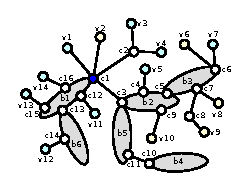
\includegraphics[width=\textwidth]{marked_bush_form_01}
  \end{minipage}
  \hfill
  \begin{minipage}[b]{0.3\textwidth}
    \includegraphics[width=\textwidth]{marked_bush_form_02}
  \end{minipage}
  \hfill
  \begin{minipage}[b]{0.3\textwidth}
    \includegraphics[width=\textwidth]{marked_bush_form_03}
  \end{minipage}
  \caption{Bush forms with the root marker on a cut vertex}\label{fig:marked_bush_form_cut_vertex}
\end{figure}


\begin{figure}[!htb]
  \centering
  \begin{minipage}[b]{0.3\textwidth}
    \includegraphics[width=\textwidth]{marked_bush_form_04}
  \end{minipage}
  \hfill
  \begin{minipage}[b]{0.3\textwidth}
    \includegraphics[width=\textwidth]{marked_bush_form_05}
  \end{minipage}
  \hfill
  \begin{minipage}[b]{0.3\textwidth}
    \includegraphics[width=\textwidth]{marked_bush_form_06}
  \end{minipage}
  \caption{Bush forms with the root marker on a block}\label{fig:marked_bush_form_block}
\end{figure}


\begin{definition}
Types of linear consecutive arrangements on the marked bush form.
\begin{itemize}
\item {\it singly partially consecutive}: the pertinent virtual nodes are arranged 
on either side of the linear order.
In figure \ref{fig:marked_bush_form_cut_vertex} left, 
($v1$, $v3$, $v4$, $v14$, $v13$, $v12$, $v11$, $v5$, $v7$, $v6$, $v8$, $v9$, $v10$, $v2$) is such an arrangement.
In figure \ref{fig:marked_bush_form_block} left, 
($v10$, $v1$, $v2$, $v14$, $v13$, $v12$, $v11$, $v3$, $v4$, $v5$, $v6$, $v7$, $v9$, $v8$) is such an arrangement.

\item {\it doubly partially consecutive}: the pertinent virtual nodes are arranged 
in the middle of the linear order.
In figure \ref{fig:marked_bush_form_cut_vertex} center,
($v2$, $v14$, $v13$, $v12$, $v11$, $v1$, $v3$, $v4$, $v5$, $v7$, $v6$, $v8$, $v9$, $v10$) is such an arrangement.
In figure \ref{fig:marked_bush_form_block} center, 
($v10$, $v11$, $v12$, $v13$, $v14$, $v1$, $v2$, $v3$, $v4$, $v5$, $v6$, $v7$, $v8$, $v9$) is such an arrangement.

\item {\it complementarily partially consecutive}: the pertinent virtual nodes are arranged on both side of
the linear order with one or more non-pertinent nodes in the middle.
In figure \ref{fig:marked_bush_form_cut_vertex} right,
($v1$, $v2$, $v3$, $v4$, $v5$, $v7$, $v6$, $v9$, $v8$, $v10$, $v11$, $v12$, $v13$, $v14$) is such an arrangement.
In figure \ref{fig:marked_bush_form_block} right, 
($v5$, $v4$, $v3$, $v2$, $v1$, $v14$, $v13$, $v12$, $v11$, $v10$, $v6$, $v7$, $v8$, $v9$) is such an arrangement.

\end{itemize}
\end{definition}

\begin{definition}
{\bf \emph{rooted embedded bc-tree}} is the underlying block-cut vertex tree of a marked bush form.
The root marker on the bush form  gives a natural root-to-descendants orientation 
on the underlying block-cut tree, and the embedding in the bush form determines
 an embedding of the block-cut tree and the embeddings of the blocks.
\end{definition}

\begin{definition}
{\bf \emph{pertinent root}} of a rooted embedded bc-tree is the highest (the closest to the root) node 
in the minimal connected subtree that spans the nodes for all the pertinent virtual nodes.
\end{definition}

The left-to-right ordering of the children of the root node is determined as follows.
If the root is for a cut vertex, then pick an arbitrary incident component of the root of the marked 
bush form,  and arrange the incident components in the counter-clock wise ordering.
If the root is for a block, then pick the incident component immediately after the marked edge in the 
counter-clock wise ordering, and arrange the incident components accordingly.


\begin{definition}
\emph{Pertinent Types} of the nodes in a rooted embedded bc-tree are recursively defined as follows.
\begin{itemize}
\item {\bf \emph{empty}}:
Each child of the node $n$ is either non-pertinent virtual edge or an empty node.
\item {\bf \emph{singly partial}}:
The node $n$ meets one of the following conditions.
\begin{itemize}
\item $n$ is for a cut vertex, there is one singly partial child, and there is no complementarily partial child.

\item $n$ is for a cut vertex, there is no singly partial child, at least one empty child, at least one full child, and no complementarily partial child.

\item $n$ is for a block, there is no complementarily partial child, there is at least one full child, all the full children are consecutively embedded on the outer face on either side of the parent with possibly at most one singly partial child at the boundary between full children and the empty ones.

\item $n$ is for a block, there is no complementarily partial child, there is no full child, and there is exactly one singly partial child immediately next to the parent.
\end{itemize}
\item {\bf \emph{doubly partial}}: 
The node $n$ meets one of the following conditions.
\begin{itemize}
\item $n$ is the pertinent root, $n$ is for a cut vertex, and there are exactly two singly partial children.
\item $n$ is the pertinent root, $n$ is for a block, at least one full child, all the full children are consecutively embedded in the middle of
 the outer face away from the parent, and possibly a singly partial child at each of the two boundaries 
between full and empty children.

\item $n$ is the pertinent root, $n$ is for a block, there is no full child,
and there are exactly two consecutively embedded singly partial children.

\end{itemize}
\item {\bf \emph{complementarily partial}}: 
The node $n$ meets one of the following conditions.
\begin{itemize}
\item $n$ is not the pertinent root, $n$ is for a cut vertex, and there are exactly two singly partial children.

\item $n$ is for a cut vertex and the children are all full except for one that is complementarily partial.

\item $n$ is for a block, and the children are arranged as the complement of the arrangement for doubly partial.

\item $n$ is for a block and the children are all full except for one that is complementarily partial.
\end{itemize}
\item {\bf \emph{full}}: 
If all the children of $n$ are either pertinent virtual edge or full.
\end{itemize}
\end{definition}

We have defined all the necessary types and operations.
Next we prove the equivalence of a PQ-tree to its bush form.


\begin{lemma}\label{lem:lemma1}
If and only if the pertinent virtual nodes in a bush form are arranged consecutively by arbitrary 
reorder and flip operations, then there is a sequence of reorder and flip operations 
on any rooted embedded bc-tree from the leaf nodes toward the root to arrange the pertinent virtual
edges in one of the linear consecutive arrangements.
At each node of the rooted embedded bc-tree, the operation is such that its children are arranged
in one of 5 pertinent types.
\end{lemma}

\begin{proof}
The details is given in Appendix \ref{App:AppendixB}.
The 'only if' part is trivial.
The 'if' part is by induction on  $|T_{BF}|$ of the rooted embedded bc-tree $T_{BF}$ of a marked bush form $BF$.
\end{proof}



We prove the equivalence between the marked bush \& its underlying rooted embedded bc-tree, 
and the PQ-tree with Lemma \ref{lem:lemma2} \& \ref{lem:lemma3} in the same induction step
 on the number of iterations of the algorithm.

\begin{lemma}\label{lem:lemma2}
Following holds for PQ-tree and its bush form:
\begin{itemize}
\item There is a one-to-one mapping between a P-node and an orienting cut vertex in the marked bush form.
\item There is a one-to-one mapping between a Q-node and an orienting block in the marked bush form.
\end{itemize}
\end{lemma}

Lemma \ref{lem:lemma2} gives the location of the marker on the marked bush form. 
If the root of the PQ-tree is a P-node, then there is a corresponding orienting cut vertex in the bush form,
and we place the marker on it.
If the root is a Q-node, there is a corresponding block $B$ in the bush form.
We place the marker on an edge $e$ of $B$ on the outer face.
The edge $e$ is determined as follows.
The children of the root Q-node in the left-to-right ordering in the PQ-tree corresponds
to a counter-clock wise ordering of the orienting active components around $B$ in the bush form.
Proceed from the cut vertex that corresponds to the right most child of the Q-node 
in the counter-clock wise orientation, find the first edge $e$ on the outer face of $B$.

\begin{lemma}\label{lem:lemma3}
   If and only if the pertinent virtual nodes in the marked bush form 
   can be consecutively arranged into one of 5 types
   using a series of reorder and flip operations from the leaves to the root,
   then there is an equivalent series of transformations by templates 
   in REDUCE() for the PQ-tree to arrange the corresponding pertinent
   leaves to the same consecutive type.
\end{lemma}

\begin{proof}
   The details of a proof of Lemma \ref{lem:lemma2} \& \ref{lem:lemma3} is given in Appendix \ref{App:AppendixC}.
   The 'only if' part is trivial. 
   The 'if' part is by induction on the number of iterations of the algorithm 
   Lemma \ref{lem:lemma3} is proved by examining exhaustively
   all the cases of operations on the marked bush form and finding equivalent templates of PQ-tree.
   Lemma \ref{lem:lemma2} is proved by examining all the cases for the births and the deaths of
   the orienting cut vertices and blocks, and find equivalent P-nodes and Q-nodes on PQ-tree. 
\end{proof}


\begin{theorem}
   If and only if the pertinent virtual edges in the bush form can be circularly consecutively arranged,
   then REDUCE() can transform the corresponding PQ-tree such that the pertinent
   leaves are arranged consecutively in one of 5 pertinent types.
\end{theorem}
\begin{proof}
   This is a direct application of Lemma 1, 2, and 3.
\end{proof}

This concludes the correctness of the new algorithm.

\section{Time Complexity}\label{se:complexity}

\begin{theorem}
   The time complexity of the new algorithm stays $O(|N|)$.
\end{theorem}
\begin{proof}
   We follow the discussion given in the original \cite{BL76} around
   Theorem 5, which depends on Lemma 2, 3 and 4 in [1].
   Lemma 2 in [1] holds for the new algorithm as there is no change in BUBBLE().

   Lemma 3 in [1] holds for the updated REDUCE() with new templates as follows.
   It's easy to see the required time for P8, Q4, and Q5 are on the order
   of the number of pertinent children. As for P7, just like P5, the empty children
   can implicitly stay in the original P-node, and it will be put under
   the new Q-node. This way, P7 runs in the order of the number of
   pertinent children.

   Lemma 4 holds for the updated REDUCE() as there are only $|S|$ leaves
   and at most $O(|S|)$ nonunary nodes in the PQ-tree.

   Theorem 5 holds as the Lemma 2, 3, and 4 hold, and also
   the new templates P7, P8, Q4, and Q5 do not apply to the unary nodes.

   In theorem 5, We substitute $m=|E|$, $n=|V|$, and $SIZE(\mathbb{S})=|E|$, and hence 
   the algorithm runs in $O(|E|+|V|+|E|) = O(|V|)$, assuming $|E| \le 3|V| -6$.
\end{proof}

\section{Implementation Issues}\label{se:implementation}
In this section we discuss two topics regarding implementation.
First we discuss the changes required to remove the pertinent tree of the complementarily partial
type. Second we propose an improvement to Ozawa-type planarization algorithms with a new
cost calculation technique.
A reference implementation is found in github:yamanishi/colameco.



\begin{figure}[!htb]
  \centering
  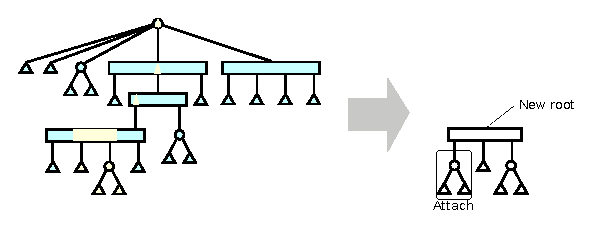
\includegraphics[width=0.7\textwidth]{pq_tree_com}
  \caption{Removal of a Complementarily Partial Pertinet Tree}
  \label{fig:pq_tree_com}
\end{figure}


Removal of a complementarily partial pertinent sub-tree and emitting new leaves
from a new P-node is different from the other cases.
A complementarily partial pertinent subtree originates from a Q-node
in template P7, or Q4. All the other nodes above this lowest Q-node including the tree root
are pertinent nodes.
They will be removed and the Q-node will become the new tree root. 
The P-node where the new leaves are attached will be put under
the Q-node on either end. See figure \ref{fig:pq_tree_com}.


There has not been a correct $O(|N|^2)$ linear time maximal planarization algorithm using PQ-tree as shown 
in \cite{JUNGER97}, except for $O(|N||E|)$ add-edge-and-test type that calls an $O(|N|)$ planarity test multiple times.
However those algorithms such as the first stage of \cite{JTS89} called
$PLANALIZE(G)$ generates a planar spanning connected subgraph and it can be used as a base graph for further maximal planarization. 
Here we base our discussion on \cite{JTS89} and propose an improvement with additional
node type and a cost value. \cite{JTS89} defines 4 node types: W, B, H, and A which correspond to
empty, full, singly partial, and doubly partial respectively. We propose a new type C which
corresponds to 'complementarily partial', and it associated cost value $c$ for each node.
The value for $c$ in $COMPUTE1()$ in \cite{JTS89} is calculated as follows.
\begin{enumerate}
\item $X$ is a pertinent leaf, $c = 0$.
\item $X$ is a full node, $c = 0$.
\item $X$ is a partial P-node, $c = a$.
\item $X$ is a partial Q-node, $c = min\{\gamma_1,\gamma_2\}$.
\end{enumerate}
\begin{equation}
\begin{aligned}
  \gamma_1 &= \sum_{i \in P(X)}(w_i) - max_{i \in P(X)}\{(w_i - c_i)\} \\
  \gamma_2 &= \sum_{i \in P(X)}(w_i) - (max_{i \in P_L(X)}\{(w_i - h_i)\}
                                       + max_{i \in P_R(X)}\{(w_i - h_i))\}
\end{aligned}
\end{equation}
where $P_L(X)$ means the maximal consecutive sequence of pertinent children of X from the
left end such that all the nodes except the right most one are full. The right most one
may be either full or singly partial. $P_R(X)$ is defined similarly from the right end.

After the cost calculation in the bottom-up manner, the type of the nodes can be determined
top-down from the tree root using the new type $C$.
In this way, the algorithm is capable of handling the complementarily partial situations, and 
would be able to reduce the number of edges removed.



\section{Experiments}\label{se:experiments}
The execution time of the new algorithm is reported in Figure \ref{fig:plot_02}.
X-axis is the time to process one graph in micro seconds taken from clock() function available on C++ standard.
Y-axis indicates the number of vertices in the given biconnected planar graph.
The test program was run on Mac 2.8GHz Corei7. 
The program was compiled by Apple LLVM 8.0.0.
The plot shows the linearity of the algorithm.

\begin{figure}[!htb]
  \centering
  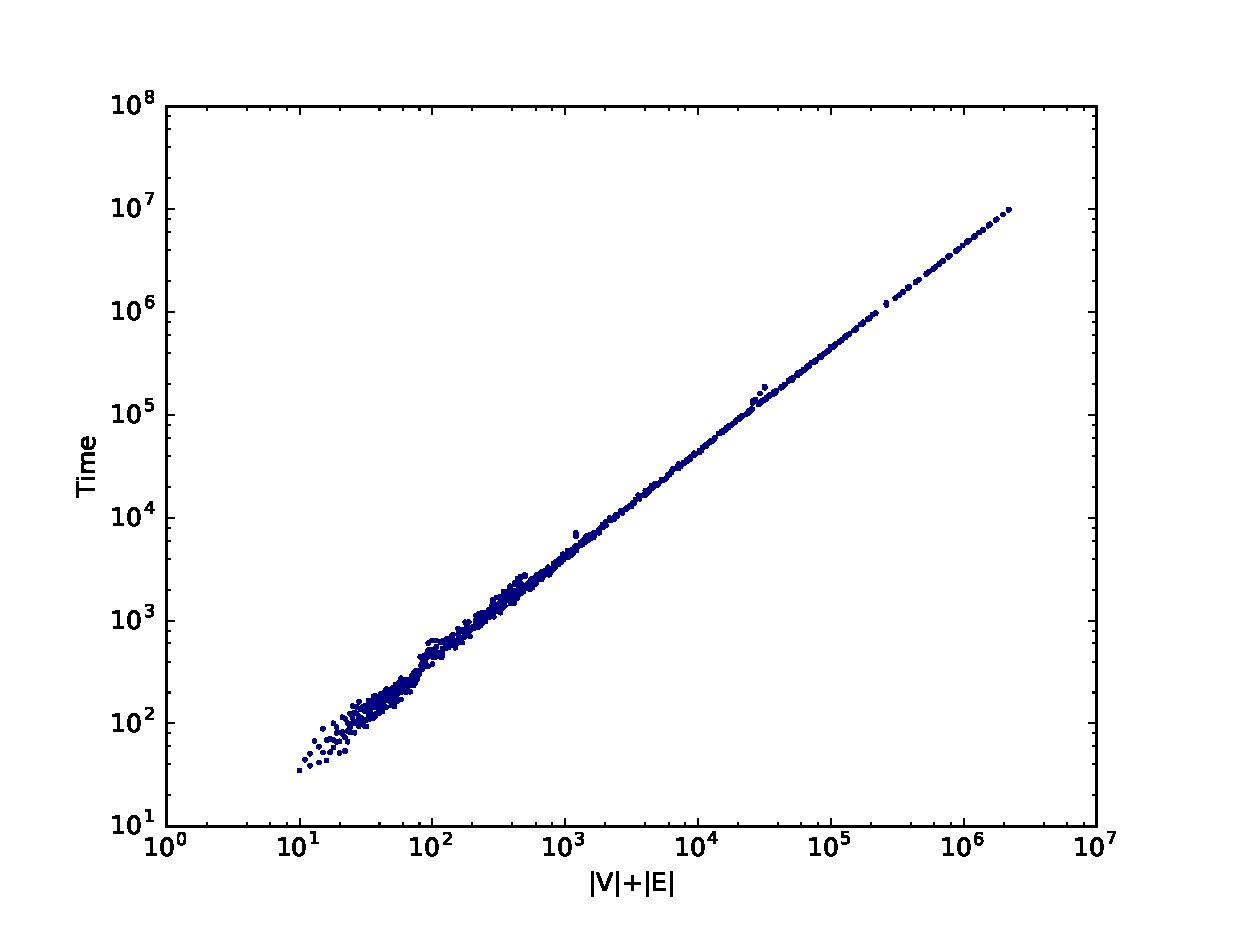
\includegraphics[width=0.8\textwidth]{plot_performance_01}
  \caption{Processing Time of the New Algorithm}
  \label{fig:plot_02}
\end{figure}


For all the test cases the new algorithm detected planarity.
Here 'ramdom'ness is not rigorous in the mathematical sense.
It is handled by the pseudo-random number generator library std::rand() and std::srand() in C++.
The code and the data used for this experiments are found in github:yamanishi/colameco.




\section{Conclusion}\label{se:conclusion}
We have shown an enhancement to the original PQ-tree planarity algorithm proposed by \cite{BL76} 
and proved the correctness. The time complexity stays in $O(|N|)$.
The enhancement applies not only to the planarity test for the graphs, but also for anything 
involving circular consecutive ones. As far as the author knows, it seems
there is no other applications than planarity testing.

\section{Acknowledgements}
The author wishes to thank whoever has encouraged and supported him for this article.

\clearpage

\bibliographystyle{abbrvurl}
\bibliography{pq_tree_enhancement}

\clearpage

% \appendix
\begin{appendices}
\section{A Planar Biconnected Graph and a ST-Numbering}\label{App:AppendixA}
Following is the planar biconnected graph and the 
st-numbering used to produce the PQ-tree and the bush form in figure 
 \ref{fig:pq_tree_01} and \ref{fig:bush_form_01}.

\begin{figure}[!htb]
  \centering
  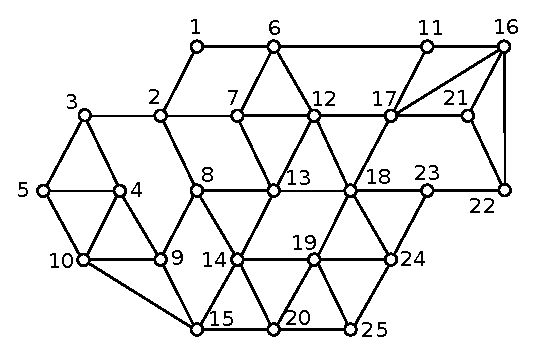
\includegraphics[width=0.5\textwidth]{sample_graph}
  \caption{Biconnected Planar Graph Used for Figure \ref{fig:pq_tree_01} and \ref{fig:bush_form_01}}
  \label{fig:sample_graph}
\end{figure}

The st-numbering:

$(8, 13, 7, 14, 19, 20, 25, 24, 23, 22, 21, 16, 11, 17, 15, 9, 10, 5, 4, 3, 2, 1, 6, 12, 18)$


\section{Proof of Lemma \ref{lem:lemma1}}\label{App:AppendixB}


The 'only if' part is trivial.  We prove the 'if' part by induction on
 $|T_{BF}|$
of the rooted embedded bc-tree $T_{BF}$ of a marked bush form $BF$.
Assume after some arbitrary reorder and flip operations, the pertinent virtual edges have been arranged
consecutively around the bush form.
This is equivalent to arranging the pertinent virtual edges into one of 5 types of 
linear consecutive arrangements in a marked bush form $BF$.
If $|T_{BF}| = 1$, the lemma trivially holds as the bush form consists of one pertinent or non-pertinent virtual node.
If $|T_{BF}| = 2$, the lemma trivially holds as the bush form consists of $k_2$ whose incident nodes are a cut vertex and a virtual node. Technically the node in $k_2$ is not a cut vertex but we consider it a cut vertex for the sake of the arguments.


Assume $|T_{BF}| \ge 3$.
We split $T_{BF}$ at the root node by splitting one connected component $C$ from the rest of $T_{BF}$.
If the marker in $BF$ is on a cut vertex $c$, then we split one connected active component $C$ of $T_{BF}$.
If the marker is on an edge $e$ of a block $B$ in $BF$, then we pick the closest cut vertex $c$ 
after $e$ in the counter-clock wise ordering around $B$ 
such that the maximal connected component after
removing the block from $c$ is still active.
Let $n_c$ be the corresponding node of $c$ in $T_{BF}$.
$C$ is the maximal connected component of $T_{BF} \setminus B$ that contains $n_c$.

Now $T_{BF}$ is decomposed into two components $D=T_{BF} \setminus C$ and $C$ at $n_c$, and
 $BF$ is decomposed into two parts $BF_{D}$ and $BF_{C}$ at $c$. 
$BF_{D}$ and $BF_{C}$ can be considered two marked bush form with the marker placed on $c$ in $BF_{C}$.
We examine each of the 5 types of linear consecutive arrangements around $BF$, 
and find all the possible combinations of pertinent types of $BF_{D}$ and $BF_{C}$.
We observe table \ref{tab:table1} enumerates all the possible combinations.
We observe for each linear consecutive arrangement around $BF$, any other
arrangements of $BF_{T\setminus C}$ or $BF_{C}$ not shown in table \ref{tab:table1} 
would lead to non-nonsecutive arrangement of the pertinent virtual nodes around $BF$.

By the induction hypothesis, the condition on the pertinent types of the children hold 
for both $BF_{D}$ and $BF_{C}$.
For each of 14 cases in Table \ref{tab:table1}, if we re-compose $BF_{D}$ and $BF_{C}$ at $c$ into $BF$, 
then we can see the condition on the corresponding pertinent type for the case holds for $BF$.
For example, if and only if $BF$ is singly partial, then there will be 6 permissible combinations of the
pertinent types of $BF_{D}$ and $BF_{C}$. We observe any other combination would leat to a different
pertinent type of $BF$ or to a non-planar arrangement.
If $BF_{D}$ ends up in full, and $BF_{C}$ in singly partial after some operations from the leaves to the root
by the induction hypothesis,
then it is easy to see that the $BF$ will end up in singly partial as desired, possibly after flipping
$BF_{C}$ and reordering all the incident component around $c$ or $B$.
The other cases can be proved in the same manner.


\begin{table}[h]
\begin {tabular}{|l|l|l|}
\hhline{|=|=|=|}
{\bf Type on $BF$} & {\bf Type on $BF_{D}$} & {\bf Type on $BF_{C}$} \\
\hhline{|=|=|=|}
Empty                   & Empty                   & Empty \\
\hhline{|=|=|=|}
Singly Partial          & Empty                   & Singly Partial \\
\hline
Singly Partial          & Empty                   & Full           \\
\hline
Singly Partial          & Singly Partial \textsuperscript{*1} & Empty     \\
\hline
Singly Partial          & Singly Partial \textsuperscript{*2} & Full  \\
\hline
Singly Partial          & Full                    & Empty          \\
\hline
Singly Partial          & Full                    & Singly Partial \\
\hhline{|=|=|=|}
Doubly Partial          & Empty                   & Doubly Partial \\
\hline
Doubly Partial          & Singly Partial \textsuperscript{*3} & Empty \\
\hline
Doubly Partial          & Singly Partial \textsuperscript{*2} & Singly Partial \\
\hline
Doubly Partial          & Doubly Partial          & Empty          \\
\hhline{|=|=|=|}
Complementarily Partial & Singly Partial \textsuperscript{*4} & Singly Partial \\
\hline
Complementarily Partial & Full                    & Complementarily Partial \\
\hhline{|=|=|=|}
Full                    & Full                    & Full \\
\hhline{|=|=|=|}
\multicolumn{3}{p{12cm}}{\textsuperscript{*1}\footnotesize{If the root is a block, then the pertinent virtual edges are on $e$ side, not on $c$ side.}}\\
\multicolumn{3}{p{12cm}}{\textsuperscript{*2}\footnotesize{If the root is a block, then the pertinent virtual edges are on $c$ side, not on $e$ side.}}\\
\multicolumn{3}{p{12cm}}{\textsuperscript{*3}\footnotesize{If the root is a block, then the pertinent virtual edges are on $c$. 
If the root is a cut vertex, this row does not apply.}}\\
\multicolumn{3}{p{12cm}}{\textsuperscript{*4}\footnotesize{If the root is a block, then the pertinent virtual edges are on $e$. If the root is a cut vertex, this row does not apply.}}\\
\end {tabular}
\caption{\textbf{All the arrangements of pertinent types of $BF_{T\setminus C}$ and $BF_{C}$.}}
\label{tab:table1}

\end{table}

\section{Proof of Lemma \ref{lem:lemma2} and \ref{lem:lemma3}}\label{App:AppendixC}


   At the first iteration, Lemma \ref{lem:lemma2} and \ref{lem:lemma3} trivially hold.
The only operation is an attach operation
   for the initial virtual edges to an initial cut vertex $c$ in the bush form,
   and the corresponding operation on PQ-tree is creation of a new P-node and attaching pertinent
   leaves to it. The root marker will be placed on $c$.

   By the induction hypothesis,  Lemma \ref{lem:lemma2},  and \ref{lem:lemma3},  hold up to $i$-th iteration.
   By Lemma \ref{lem:lemma1} and \ref{lem:lemma2},
   there is a marked bush form $BF$ whose marker is placed on a cut vertex $c$ if
   the root of the PQ-tree is P-node, or on an edge of a block $B$ if the root is a Q-node.
   Assume we have arranged the pertinent nodes for the $i+1$-th iteration by an arbitrary set
   of reorder and flip operations on the bush form.
   Then by Lemma \ref{lem:lemma1}, 
   we can arrange the child components of each node of the rooted embedded bc-tree $T_{BF}$
   into one of 5 pertinent types from the descendants toward the root in $T_{BF}$.

   Now we examine each pertinent type for a cut vertex and a block in a marked bush form
   for their equivalence to their
   corresponding nodes in the PQ-tree. We introduce two new operations to the marked bush form, which
   are interlock and split.
   Table \ref{tab:table2} shows all the operations on an orienting cut vertex 
   and their equivalent templates on PQ-tree.
   Table \ref{tab:table3} is for an orienting block.

   Following explains the symbols used in those tables.
   \begin {itemize}
   \item a square is a component
   \item a circle is a cut vertex
   \item sky blue indicates pertinent component.
   \item yellow indicates non-pertinent component.
   \item a square enclosing '$p$' is a parent bock component. 
This does not apply if the cut vertex is the root.
   \item a circle enclosing '$p$' is a parent cut vertex component.
This does not apply if the block is the tree root.
   \item a square in sky blue is a full component.
   \item a square in yellow is a non-pertinent component.
   \item a rectangle enclosing yellow and sky blue squares is a singly partial component.
   \item a circle is in sky blue with a yellow wedge is a complementarily partial component.
   \item a polygon is a block.
   \item a grey triangle or a quadrilateral is a block induced by a split operation at a cut vertex.
   \item a dashed broken line indicates interlocking of two blocks.
   \end {itemize}

   We observe the rows of those tables cover exhaustively all the cases of 4 pertinent types. (Empty type
   is not considered.)
   Then we can prove the equivalence for each case with the aid of interlock and split operations
   as well as reorder and flip.
   For example, take the case for 'Singly Partial 2' for an orienting cut vertex $c$.
   Originally, $c$
   has 3 full child components, 3 non-pertinent child components, and a singly partial child component.
   To make it singly partial, we first reorder the incident ordering of those children so that
   the full children are arranged consecutively on one side, the non-pertinent children on the other,
   and the singly partial child between those two oriented such that the full side of the singly partial
   child is on the full side of children. Please note it is not a circular ordering due to the presence
   of the parent component.
   To make those changes permanent, we split $c$
   to a triangle $k_3$ or a qiadrilateral $C_4$ and fix the orientation of the singly partial child
   relative to them with the interlock operation. The 3rd column in Table \ref{tab:table2} is for the case
   if $c$ is a root component, and the 5th column is for the case if it is not.
   We can see those are in fact equivalent to the template P4 and P5 respectively for the case in which
   the are both full and non-pertinent components.
   In the 3rd column, the interlocked $k_3$ and the singly partial child together correspond to 
   the resultant Q-node in P4 with the orientation of the children preserved. If there are more than 1
   full child component, the full vertex on $k_3$ becomes a new orienting cut vertex, which corresponds
   to the new full P-node under the Q-node in P4.  Similarly, in the 5th column, the interlocked $C_4$
   and the singly partial child together correspond to the resultant Q-node in P5.
   The other cases can be examined in the same way.
   We see that in fact, those tables cover all the cases for all the templates for PQ-tree.
    In case of 'Doubly Partial 4', there are no corresponding PQ-tree templates, as those nodes are above the 
   pertinent root.
   This concludes the proof of Lemma 3.

   As for Lemma 2, we prove the equivalence in the birth and the death of the orienting cut vertex
   and the corresponding P-node, and the equivalence of an orienting block to Q-node.

   An orienting cut vertex is born only at the following location.
   \begin{itemize}
   \item an attach operation with more than 1 virtual edge to be attached.
   \end{itemize}

   Please note that a split operation can produce $k_3$ or $C_4$, which means 2 or 3 new cut vertices
   are created. However, the one incident to the parent is not orienting as it has just 2 active components.
   The one incident to the interlocked singly partial child is not orienting either.
   The one on the full side is a temporary cut vertex which will be absorbed inside a newly created 
   block on a merge operation later. The remaining one on the non-pertinent side is considered to have been
   transferred from the original cut vertex. So, effectively a split operation does not create new orienting cut vertex.

   An orienting cut vertex will die at the following locations.
   \begin{itemize}
   \item Becoming full. In this case the children of the cut vertex will be merged into a new cut vertex,
   and eventually it will have two active components and will become non-orienting.

   \item Becoming complementarily partial, and it has a complementarily partial child.
   In this case all the full children together with the parent will be merged into a new cut vertex,
   and eventually it will have two active components and will become non-orienting.

   \item Singly Partial 1, non-pertinent root, and there is one non-pertinent child. In this case the new cut vertex
   on the non-pertinent side of $k_3$ will have only one child, and it has two active components and it 
   will become non-orienting.

   \item Singly Partial 3, non-pertinent root, and there is one non-pertinent child. In this case the new cut vertex
   on the non-pertinent side of $k_3$ will have only one child, and it has two active components and it 
   will become non-orienting.

   \item Singly Partial 4, pertinent root and non-pertinent root, and there is no non-pertinent child. In this case, the $k_3$ by the split
   operation does not produce any cut vertex for non-pertinent children and hence the cut vertex vanish.

   \item Doubly Partial or Complementarily Partial 3, Root and Non-root, and there is no non-pertinent child. 
In this case, the $C_4$ by the split
   operation does not produce any cut vertex for non-pertinent children and hence the cut vertex vanish.
   \end{itemize}

   An orienting block is born at the following conditions.
   \begin{itemize}
   \item $k_3$ or $C_4$ is generated by a split operation
   \end{itemize}

   An orienting block dies at the following locations.
   \begin{itemize}
   \item Where a singly partial child is interlocked to the parent. In this case there is a singly
   partial block in the component specified by the singly partial child, and the parent.
   \item Becoming full. In this case the children of the block will be merged into a new cut vertex,
   and eventually it will have two active components and will become non-orienting.

   \item Becoming complementarily partial, and it has a complementarily partial child.
   In this case all the full children together with the parent will be merged into a new cut vertex,
   and eventually it will have two active components and will become non-orienting.
   \end{itemize}

   For each of the birth and death cases above, there is a corresponding creation or destruction of 
   P-node or Q-node. For example, take the 3rd death case of an orienting cut vertex that is a singly
   partial and non-root and that has one non-pertinent child. This corresponds to template P3.
   Since there is one non-pertinent child, it will be directly placed as one of two children of the Q-node.
   Eventually, the original P-node is considered removed from the PQ-tree.
   We can show the equivalence for the other cases. We can also show those cases cover all the locations
   in the templates, attach and removal of the pertinent subtree in which new P-nodes and Q-nodes are created
   and destructed. This concludes the proof of Lemma \ref{lem:lemma2}.

\begin{table}[h]
  \def\arraystretch{1}
  \centering
  \begin{tabular}
      {|C{0.22\textwidth}|C{0.14\textwidth}|C{0.14\textwidth}|C{0.05\textwidth}|C{0.14\textwidth}|C{0.05\textwidth}|}
      \hline 
      Pertinent type & Original State & Operation for Pert Root & PQ Op. & Operation for Non-Pert Root & PQ Op.\\
      \hline
      Full&
      \includegraphics[width=0.1\textwidth]{bc_transform_cv_01_before} &
      \includegraphics[width=0.1\textwidth]{bc_transform_cv_01_root} &
      P1 &
      \includegraphics[width=0.1\textwidth]{bc_transform_cv_01_nonroot} &
      P1 \\
      \hline
      Empty &
      \includegraphics[width=0.1\textwidth]{bc_transform_cv_11_before} &
      \includegraphics[width=0.1\textwidth]{bc_transform_cv_11_root} &
      - &
      \includegraphics[width=0.1\textwidth]{bc_transform_cv_11_nonroot} &
      - \\
      \hline
      Singly Partial 1&
      \includegraphics[width=0.1\textwidth]{bc_transform_cv_02_before} &
      \includegraphics[width=0.1\textwidth]{bc_transform_cv_02_root} &
      P2 & 
      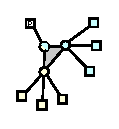
\includegraphics[width=0.1\textwidth]{bc_transform_cv_02_nonroot} &
      P3 \\
      \hline
      Singly Partial 2& 
      \includegraphics[width=0.1\textwidth]{bc_transform_cv_03_before} &
      \includegraphics[width=0.1\textwidth]{bc_transform_cv_03_root} &
      P4 &
      \includegraphics[width=0.1\textwidth]{bc_transform_cv_03_nonroot} &
      P5 \\
      \hline
      Singly Partial 3& 
      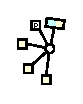
\includegraphics[width=0.1\textwidth]{bc_transform_cv_04_before} &
      N/A&
      - &
      \includegraphics[width=0.1\textwidth]{bc_transform_cv_04_nonroot} &
      P5 \\
      \hline
      Singly Partial 4& 
      \includegraphics[width=0.1\textwidth]{bc_transform_cv_05_before} &
      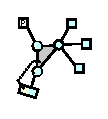
\includegraphics[width=0.1\textwidth]{bc_transform_cv_05_root} &
      P4 &
      \includegraphics[width=0.1\textwidth]{bc_transform_cv_05_nonroot} &
      P5 \\
      \hline
      Doubly Partial or Complementarily Partial 1&
      \includegraphics[width=0.1\textwidth]{bc_transform_cv_06_before} &
      \includegraphics[width=0.1\textwidth]{bc_transform_cv_06_root} &
      P6 &
      \includegraphics[width=0.1\textwidth]{bc_transform_cv_06_nonroot} &
      P7 \\
      \hline
      Doubly Partial or Complementarily Partial 2&
      \includegraphics[width=0.1\textwidth]{bc_transform_cv_07_before} &
      \includegraphics[width=0.1\textwidth]{bc_transform_cv_07_root} &
      P6 &
      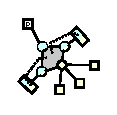
\includegraphics[width=0.1\textwidth]{bc_transform_cv_07_nonroot} &
      P7 \\
      \hline
      Doubly Partial or Complementarily Partial 3&
      \includegraphics[width=0.1\textwidth]{bc_transform_cv_08_before} &
      \includegraphics[width=0.1\textwidth]{bc_transform_cv_08_root} &
      P6 &
      \includegraphics[width=0.1\textwidth]{bc_transform_cv_08_nonroot} &
      P7 \\
      \hline
      Doubly Partial 4&
      \includegraphics[width=0.1\textwidth]{bc_transform_cv_10_before} &
      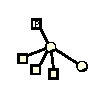
\includegraphics[width=0.1\textwidth]{bc_transform_cv_10_root} &
      - &
      \includegraphics[width=0.1\textwidth]{bc_transform_cv_10_nonroot} &
      - \\
      \hline
      Complementarily Partial&
      \includegraphics[width=0.1\textwidth]{bc_transform_cv_09_before} &
      \includegraphics[width=0.1\textwidth]{bc_transform_cv_09_root} &
      P8 &
      \includegraphics[width=0.1\textwidth]{bc_transform_cv_09_nonroot} &
      P8 \\
      \hline



 \end{tabular}
 \caption{Operations on an orienting cut vertex and equivalent PQ-tree templates}
 \label{tab:table2}
\end{table}


\begin{table}[h]
  \def\arraystretch{1}
  \centering
  \begin{tabular}
      {|C{0.22\textwidth}|C{0.14\textwidth}|C{0.14\textwidth}|C{0.05\textwidth}|C{0.14\textwidth}|C{0.05\textwidth}|}
      \hline 
      Pertinent type & Original State & Operation for Pert Root & PQ Op. & Operation for Non-Pert Root & PQ Op.\\
      \hline
      Full&
      \includegraphics[width=0.1\textwidth]{bc_transform_bl_01_before} &
      \includegraphics[width=0.1\textwidth]{bc_transform_bl_01_root} &
      Q1 &
      \includegraphics[width=0.1\textwidth]{bc_transform_bl_01_nonroot} &
      Q1 \\
      \hline
      Empty&
      \includegraphics[width=0.1\textwidth]{bc_transform_bl_12_before} &
      \includegraphics[width=0.1\textwidth]{bc_transform_bl_12_root} &
      - &
      \includegraphics[width=0.1\textwidth]{bc_transform_bl_12_nonroot} &
      - \\
      \hline
      Singly Partial 1&
      \includegraphics[width=0.1\textwidth]{bc_transform_bl_02_before} &
      \includegraphics[width=0.1\textwidth]{bc_transform_bl_02_root} &
      Q2 & 
      \includegraphics[width=0.1\textwidth]{bc_transform_bl_02_nonroot} &
      Q2 \\
      \hline
      Singly Partial 2& 
      \includegraphics[width=0.1\textwidth]{bc_transform_bl_03_before} &
      \includegraphics[width=0.1\textwidth]{bc_transform_bl_03_root} &
      Q2 &
      \includegraphics[width=0.1\textwidth]{bc_transform_bl_03_nonroot} &
      Q2 \\
      \hline
      Doubly Partial 1& 
      \includegraphics[width=0.1\textwidth]{bc_transform_bl_04_before} &
      \includegraphics[width=0.1\textwidth]{bc_transform_bl_04_root} &
      Q3 &
      N/A &
      - \\
      \hline
      Doubly Partial 2& 
      \includegraphics[width=0.1\textwidth]{bc_transform_bl_05_before} &
      \includegraphics[width=0.1\textwidth]{bc_transform_bl_05_root} &
      Q3 &
      N/A &
      - \\
      \hline
      Doubly Partial 3& 
      \includegraphics[width=0.1\textwidth]{bc_transform_bl_06_before} &
      \includegraphics[width=0.1\textwidth]{bc_transform_bl_06_root} &
      Q3 &
      N/A &
      - \\
      \hline
      Doubly Partial 4& 
      \includegraphics[width=0.1\textwidth]{bc_transform_bl_11_before} &
      \includegraphics[width=0.1\textwidth]{bc_transform_bl_11_nonroot} &
      - &
      \includegraphics[width=0.1\textwidth]{bc_transform_bl_11_root} &
      - \\
      \hline
      Complementarily Partial 1& 
      \includegraphics[width=0.1\textwidth]{bc_transform_bl_07_before} &
      N/A &
      - &
      \includegraphics[width=0.1\textwidth]{bc_transform_bl_07_nonroot} &
      Q4 \\
      \hline
      Complementarily Partial 2& 
      \includegraphics[width=0.1\textwidth]{bc_transform_bl_08_before} &
      N/A &
      - &
      \includegraphics[width=0.1\textwidth]{bc_transform_bl_08_nonroot} &
      Q4 \\
      \hline
      Complementarily Partial 3& 
      \includegraphics[width=0.1\textwidth]{bc_transform_bl_09_before} &
      N/A &
      - &
      \includegraphics[width=0.1\textwidth]{bc_transform_bl_09_nonroot} &
      Q4 \\
      \hline
      Complementarily Partial 4& 
      \includegraphics[width=0.1\textwidth]{bc_transform_bl_10_before} &
      N/A &
      - &
      \includegraphics[width=0.1\textwidth]{bc_transform_bl_10_nonroot} &
      Q5 \\
      \hline

 \end{tabular}
 \caption{Operations on an orienting block and equivalent PQ-tree templates}
 \label{tab:table3}
\end{table}


\end{appendices}

\end{document}




